\section{Auswertung}
\subsection{Isobare Molwärme}
Um die Molwärme bei konstantem Druck aus den gegebenen Messwerten zu bestimmen, muss zunächst die Zeitdifferenz für alle gemessenen Zeiten bestimmt werden. Aus dieser kann dann die elektrische Energie mit der Formel

\begin{equation}
E=U\cdot I\cdot\Delta t
\end{equation}

berechnet werden. Dann wird die Temperatur aus dem Widerstand mit Hilfe der Formel 

\begin{equation}
T=0,00134\cdot R^2+2,296\cdot R-243,02
\end{equation}

bestimmt. Mit diesen Werten kann nun die spezifische Wärme berechnet werden. Da hier die Molwärme betrachtet wird, muss die spezifische Wärme lediglich mit dem Verhältnis aus dem molekular Gewicht zur Gesamtmasse multipliziert werden wie in Formel

\begin{equation}
C_p=\frac{m_\text{mol}}{m}\frac{E}{\Delta T}\quad.
\end{equation}

\noindent Die benutzten Messwerte sind Tabelle \ref{fig:tab1} zu entnehmen.   

\begin{table}[H]
	\begin{center}
		\begin{tabular}{c c c c c c}
			\toprule
			\(t\)/s & \(R\)/\(\Omega\) & \(I\)/mA & \(U\)/V & \(T\)/K & \(\sigma_T\) \\
			\midrule
			0		&22,2		&133,9	&14,14	&81,76	&0,24 \\
			300		&25,2		&136,0	&14,24	&88,84	&0,24 \\
			600		&27,6		&146,1	&15,32	&94,52	&0,24 \\
			900		&30,0		&160,0	&16,79	&100,22	&0,24 \\
			1200	&33,1		&166,4	&17,48	&107,60	&0,24 \\
			1500	&36,2		&175,7	&18,49	&115,00	&0,24 \\
			1800	&39,2		&180,3	&18,98	&122,19	&0,24 \\
			2100	&44,9		&180,8	&18,98	&135,92	&0,24 \\
			2400	&48,8		&180,0	&18,98	&145,37	&0,24 \\
			2700	&52,7		&180,3	&18,98	&154,85	&0,24 \\
			3000	&56,3		&180,4	&18,98	&163,64	&0,24 \\
			3300	&59,8		&180,5	&18,98	&172,22	&0,25 \\
			3600	&63,3		&180,6	&18,98	&180,84	&0,25 \\
			3900	&66,6		&180,7	&18,98	&188,99	&0,25 \\
			4260	&70,4		&180,8	&18,98	&198,41	&0,25 \\
			4620	&73,3		&180,9	&18,98	&205,63	&0,25 \\
			4980	&77,8		&181,0	&18,98	&216,87	&0,25 \\
			5340	&81,0		&181,0	&18,98	&224,89	&0,25 \\
			5760	&85,6		&181,1	&18,98	&236,48	&0,25 \\
			6120	&89,0		&181,1	&18,98	&245,09	&0,25 \\
			6480	&92,5		&181,2	&18,98	&253,98	&0,25 \\
			6840	&96,1		&181,2	&18,98	&263,15	&0,26 \\
			7200	&99,7		&181,3	&18,98	&272,36	&0,26 \\
			7560	&102,5		&181,3	&18,98	&279,55	&0,26 \\
			7980	&106,6		&181,3	&18,98	&290,11	&0,26 \\
			8400	&110,2		&181,3	&18,98	&299,42	&0,26 \\
			\bottomrule
		\end{tabular}
		\caption{Messdaten und Temperatur}
		\label{fig:tab1}
	\end{center}
\end{table}

\noindent Hierbei wird für die Zeit ein Reaktionsfehler von \(\sigma_t=1\text{s}\), für den Widerstand ein Ablesefehler von \(\sigma_\Omega=0,1\text{Ohm}\) und für Strom und Spannung jeweils ein Ablesefehler von \(\sigma_I=0,01\text{mA}\) und \(\sigma_U=0,01\text{V}\) angenommen.

\noindent Da in der Molwärme und Energie Differenzen auftreten, wird der letzte Messwert nicht mehr in die Berechnung eingehen.

\noindent Die Messunsicherheit der Energie berechnet sich aus der Formel für die Gauß'sche Fehlerfortpflanzung:

\begin{equation}
\sigma_E=\sqrt{(I\Delta t\cdot\sigma_U)^2 + (U\Delta t\cdot\sigma_I)^2 + (UI\cdot\sigma_t)^2}
\end{equation}

\noindent Die Messunsicherheit für die Molwärme ebenso:

\begin{equation}
\sigma_{C_p}=\sqrt{\left(\frac mM\cdot\frac{1}{\Delta t}\cdot\sigma_E\right)^2+\left(-\frac mM\cdot\frac{E}{\Delta t^2}\cdot\sigma_t\right)^2 }
\end{equation}

\noindent Die Ergebnisse für die Molwärme und Energie sind Tabelle \ref{fig:tab2} zu entnehmen.

\begin{table}[H]
	\begin{center}
		\begin{tabular}{c c c c c c}
			\toprule
			\(E\)/J & \(\sigma_E\) & \(\Delta t\)/s & \(\Delta T\)/K & \(C_p\)/\(\frac{\text{J mol}}{\text{K}}\) & \(\sigma_{C_p}\) \\
			\midrule
			568,00	&2,68	&300	&81,76	&14,91	&0,71\\
			580,99	&2,74	&300	&88,84	&19,00	&1,12\\
			671,48	&3,17	&300	&94,52	&21,91	&1,30\\
			805,92	&3,79	&300	&100,22	&20,29	&0,93\\
			872,60	&4,11	&300	&107,59	&21,89	&1,00\\
			974,61	&4,59	&300	&115,00	&25,18	&1,19\\
			1026,62	&4,84	&300	&122,19	&13,89	&0,35\\
			1029,48	&4,85	&300	&135,92	&20,26	&0,74\\                           
			1024,92	&4,83	&300	&145,37	&20,08	&0,86\\
			1026,63	&4,84	&300	&154,85	&21,69	&0,86\\ 
			1027,20	&4,84	&300	&163,64	&22,24	&0,90\\
			1027,76	&4.85	&300	&172,22	&22,17	&0,90\\
			1028,34	&4,85	&300	&180,84	&23,44	&1,01\\
			1234,69	&4,85	&360	&188,99	&24,35	&0,91\\
			1235,37	&4,85	&360	&198,41	&31,81	&1,56\\
			1236,05	&4.86	&360	&205,63	&20,43	&0,65\\
			1236,74	&4.86	&360	&216,87	&28,63	&1,27\\                
			1442,86	&4.86	&360	&224,89	&23,14	&0,76\\                  
			1237,42	&4.86	&360	&236,40	&26,73	&1,12\\                    
			1237,42	&4.86	&360	&245,09	&25,87	&1,05\\
			1238,10	&4.86	&360	&253,98	&25,07	&0,98\\ 
			1238,10	&4.86	&360	&263,15	&24,97	&0,99\\            
			1238,78	&4.86	&360	&272,36	&32,02	&1,62\\
			1445,25	&4.86	&420	&279,55	&25,43	&0,88\\
			1445,25	&4.86	&420	&290,11	&28,84	&1,14\\
			\bottomrule
		\end{tabular}
		\caption{Energie und Molwärme}
		\label{fig:tab2}
	\end{center}
\end{table}

\subsection{Isochore Molwärme}
Die Molwärme bei konstantem Volumen wird über die Korrekturformel

\begin{equation}
C_V=C_p-9\alpha^2\kappa V_0T
\end{equation}

berechnet. Hierzu ist das Wissen über die Werte des Ausdehnungskoeffizienten von Relevanz. In Abbildung \ref{fig:abb1} sind Werte für \(\alpha\) für bestimmte Temperaturen angegeben.

\begin{figure}
	\centering
		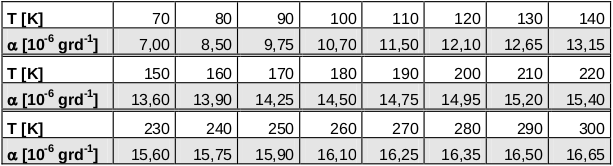
\includegraphics[width=0.5\textwidth]{alpha.png}
	\caption{Ausdehnungskoeffizent für bestimmte Temperaturen}
	\label{fig:abb1}
\end{figure}

\noindent Um Werte für die gegebenen Temperaturen aus Tabelle \ref{fig:tab1} zu bekommen, werden die Werte aus Tabelle \ref{fig:tab3} als Stützstellen mit Hilfe eines Polynoms sechsten Grades interpoliert. 

\noindent Für die Korrekturformel wird noch der Kompressionsmodul und das Molvolumen benötigt. Hierfür werden Literaturwerten verwendet: \(\kappa=1,378\cdot10^{11}\frac{\text{N}}{\text{m}^2}\), \(V_0=7,11\cdot10^{-6}\frac{\text{m}^3}{\text{mol}}\). 

\noindent Die Werte für die Molwärme und die passenden Ausdehnungskoeffizienten sind der Tabelle \ref{fig:tab4} zu entnehmen.

\begin{table}[H]
	\begin{center}
		\begin{tabular}{c c c}
			\toprule
			\(\alpha/\text{K}\cdot10^{-6}\) & \(C_V\)/\(\frac{\text{J mol}}{\text{K}}\) & \(\sigma_{C_V}\) \\
			\midrule
			8,75		&14,85	&0,72\\
			9,59		&18,93	&1,14\\
			10,18	&21,82	&1,33\\
			10,71	&20,19	&1,01\\
			13,10	&21,77	&1,13\\
			11,82	&25,04	&1,38\\
			12,27	&13,73	&0,95\\
			12,97	&20,05	&1,56\\
			13,37	&19,85	&1,97\\
			13,73	&21,44	&2,54\\
			14,02	&21,96	&3,16\\
			14,29	&21,86	&3,89\\
			14,52	&23,10	&4,80\\
			14,73	&23,98	&5,79\\
			14,95	&31,41	&7,30\\
			15,11	&20,01	&8,42\\
			15,34	&28,17	&10,82\\
			15,49	&22,66	&12,76\\
			15,69	&26,21	&16,21\\
			15,84	&25,33	&19,22\\
			15,98	&24,50	&22,84\\
			16,12	&24,37	&27,18\\
			16,26	&31,39	&32,25\\
			16,37	&24,76	&36,70\\
			16,51	&28,14	&44,23\\
			\bottomrule
		\end{tabular}
		\caption{Ausdehnungskoeffizient für gemessene Temperaturen und Molwärme bei konstantem Volumen}
		\label{fig:tab3}
	\end{center}
\end{table}

\noindent Die Molwärme bei konstantem Volumen gegen die Temperatur im linearen Diagramm wird in Abbildung \ref{fig:abb2} dargestellt.

\begin{figure}
	\centering
		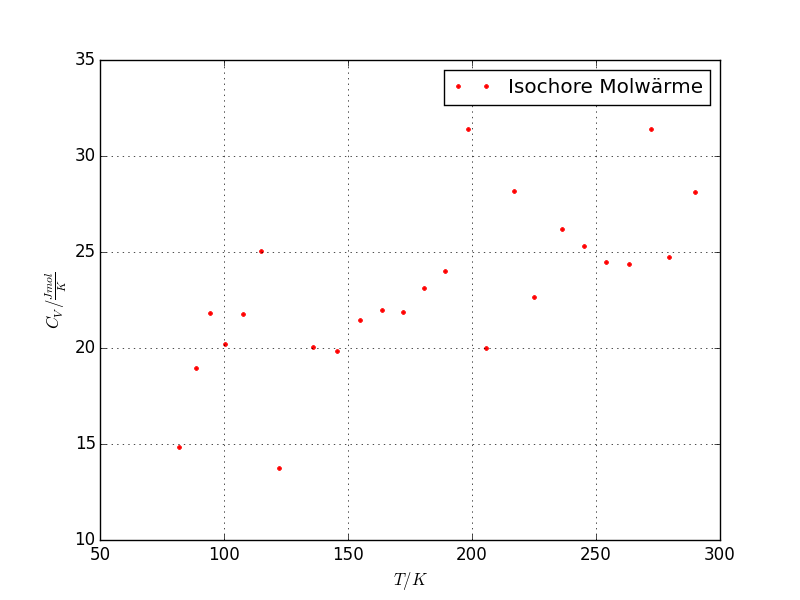
\includegraphics[width=0.5\textwidth]{cv.png}
	\caption{Molwärme über Temperatur}
	\label{fig:abb2}
\end{figure}

\subsection{Debye-Temperatur}
Die Debye-Temperatur wird aus der Molwärme bei konstantem Volumen und der Temperaturen bis zu 170K bestimmt, indem die Werte der Molwärme an die, aus Abbildung \ref{fig:abb3} angepasst werden. Die Zahlen der linken Spalte bilden dabei die Mantisse und die Zahlen der oberen Zeile die Werte für \(\frac{\theta_\text{D}}{T}\). Die Debye-Temperatur wird dann durch Multiplikation mit der Temperatur berechnet. Das Ergebnis ist Tabelle \ref{fig:tab4} zu entnehmen.

\begin{figure}
	\centering
		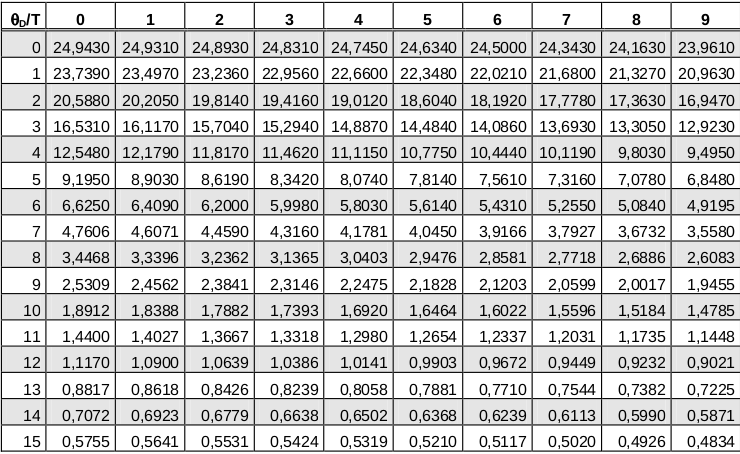
\includegraphics[width=0.5\textwidth]{debye.png}
	\caption{Debye-Temperatur für bestimmte Molwärme}
	\label{fig:abb3}
\end{figure}

\begin{table}[H]
	\begin{center}
		\begin{tabular}{c c c c}
			\toprule
			\(T\)/K & \(C_V\)/\(\frac{\text{J mol}}{\text{K}}\) & \(\frac{\theta_\text{D}}{T}\) & \(\theta_D\)/K \\
			\midrule
			81,76	&14,85	&3,4		&277,98\\
			88,84	&18,93	&2,4		&213,22\\
			94,52	&21,82	&1,7		&160,68\\
			100,22	&20,19	&2,1		&210,46\\
			107,60	&21,77	&1,7		&182,92\\
			115,00	&25,04	&0,0		&0,00\\
			122,19	&13,73	&1,8		&219,94\\
			135,93	&20,05	&1,6		&217,47\\
			145,37	&19,85	&1,7		&247,13\\
			154,85	&21,44	&1,2		&185,82\\
			163,64	&21,96	&0,9		&147,28\\
			\bottomrule
		\end{tabular}
		\caption{Debye-Temperatur Anpassung}
		\label{fig:tab4}
	\end{center}
\end{table}

\noindent Der Mittelwert dieser Werte für die Debye-Temperatur lautet:

\begin{equation}
\frac{1}{11}\sum\limits_{i=1}^{11}{\theta_{\text{D}}}_i=\overline{\theta_\text{D}}=187,54
\end{equation}

\noindent Die Standardabweichung ist dann:

\begin{equation}
\sigma_\theta=\sqrt{\frac{1}{10}\sum\limits_{i=1}^{11}({\theta_{\text{D}}}_i-\overline \theta_{\text{D}})^2}=21,83
\end{equation}

\subsection{Debye-Frequenz}
Zur Berechnung der theoretischen Debye-Frequenz wird die Forderung

\begin{equation}
\int\limits_0^{\omega_\text{D}}D(\omega)\text{d}\omega=3N_L
\end{equation}

betrachtet. Aus dieser folgt der Ausdruck:

\begin{equation}
\omega_\text{D}=\sqrt[3]{\frac{18\pi^2N_L}{L^3}\frac{1}{\left(\frac{1}{v_{\text{long}}^3}+\frac{1}{v_\text{trans}^3}\right)}}
\end{equation}

mit dem es möglich ist, die Debye-Frequenz analytisch zu bestimmen.

\noindent Die noch zu bestimmenden Größen sind die Anzahl der Freiheitsgrade und das Volumen der Probe.

\begin{equation*}
N_L=\frac{m}{m_\text{Atom}}=\frac{0,342\text{kg}}{63,55\cdot 1,66\cdot10^{-27}\text{kg}}=3,24\cdot10^{24}
\end{equation*}

\begin{equation*}
L^3=\frac{m}{\rho_\text{Kupfer}}=\frac{0,342\text{kg}}{8,92\cdot10^3\frac{kg}{\text{m}^3}}=3,83\cdot10^{-5}\text{m}^3
\end{equation*}

\noindent Dabei ist \(m_\text{Atom}\) die Masse eines einzelnen Kupferatoms. Für die Geschwindigkeiten wird \(v_\text{long}=4,7\cdot10^3\frac{\text{m}}{\text{s}}\) und \(v_\text{trans}=2,26\cdot10^3\frac{\text{m}}{\text{s}}\) verwendet.

\noindent Daraus ergibt sich für die Debye-Frequenz:

\begin{equation*}
\omega_\text{D}=5,38\cdot10^{13}\frac{1}{\text{s}}
\end{equation*}

\noindent Daraus lässt sich auch die theoretische Debye-Temperatur berechnen. Mit Formel

\begin{equation}
\theta_\text{D}=\frac{\hbar\omega_\text{D}}{k_\text{B}}
\end{equation}

lautet die theoretische Temperatur:

\begin{equation*}
\theta_\text{D}=411,22\text{K}
\end{equation*}